\chapter{Resultater}
\section{Del 1}
\subsection{Oppgave 1}
\(\begin{tabular}{|c|c|c|c|}
    \hline
    \#&Funksjonsuttrykk $f(x)$ & Intervall & $x_{0}$ \\
     \hline
     1&$f(x)=7x^{2}-8x+1$    &   $0 \leq x \leq 2$    &$    x_{0} = 1$\\
     \hline
     2&$f(x)=sin(x)$      &   $0 \leq x \leq 2\pi$      &       $x_{0} = \pi/4$\\
     \hline
     3&$f(x)=\frac{1-x}{(x+3)^{2}}$&$-1\leq x \leq 2$&$x_{0} = 1$\\
     \hline
     4&$f(x)=\sqrt{1+x^{2}}$&$0 \leq x \leq 10$&$x_{0} = 5$ \\
     \hline
\end{tabular}\)\\
\subsubsection{A)}
    Finn den deriverte $f'(x)$ (ikke en tilnærming) ved å bruke kjente regler for derivasjon.
    \begin{enumerate}
        \item $f'(x)=14x-8$
        \item $f'(x)=cos(x)$
        \item $f'(x)=\frac{x-5}{(x+3)^{3}}$
        \item $f'(x)=\frac{x}{\sqrt{(1+x)^{2}}}$
    \end{enumerate}
\subsubsection{B)}
    Regn ut $f'(x_{0})$, samt en tilnærming ved å gjøre bruk av $g(x)$ fra (2) med $\Delta x = 0.1$.\\
    \bgroup
    \def\arraystretch{2}
    \begin{tabular}{|c|l|l|}
    \hline
    1& $f'(x_{0})=14(1)-8=6$&$g(1)=\frac{(7*1.1^2-8*1.1+1)-(7*1-8*1+1)}{0.1}\approx{6.7}$\\
    \hline
    2& $f'(x_{0})=cos(\frac{\pi}{4})=\frac{\sqrt{2}}{2}\approx{0.71}$&$g(\frac{\pi}{4})=\frac{sin(0.885)-sin(\frac{\pi}{4})}{0.1}\approx{0.67}$\\
    \hline
    3& $f'(x_{0})=\frac{1-5}{(1+3)^2}=-\frac{1}{16}$&$g(1)=\frac{{}\frac{1-1.1}{(1.1+3)^2} - \frac{1-1}{(1+3)^2}}{0.1}\approx{-0.059}$\\
    \hline
    4& $f'(x_{0})=\frac{5}{\sqrt{1+5^2}}=\frac{5\sqrt{26}}{26}$&$g(5)=\frac{\sqrt{1+5.1^2}-\sqrt{1+5^2}}{0.1}\approx{0.981}$\\
    \hline
    \end{tabular}
    \egroup
\subsubsection{C)}
    Beregn E(x$_{0}$).
    \begin{enumerate}
        \item $E(x_{0})=|6-6.7|=0.7$
        \item $E(x_{0})=|0.7071-0.67|=0.0371$
        \item $E(x_{0}=|0.062-0.059|=0.003$
        \item $E(x_{0}=|0.9805-0.981|=0.005$
    \end{enumerate}
\subsubsection{D)}
Finn, ved prøving og feiling, den største $\Delta$x avrundet til to signifikante desimaler, slik at $E(x_{0}) \leq 0.001$.
\\
$\Delta$x verdiene her ble funnet ved hjelp av et python program. Utklipp mellom hvert listepunkt for hver funksjon. Se vedlegg for kode. Vedlegg: \ref{app:func1}. Web: \cite{github}
\begin{enumerate}
    \item $E\leq 0.001$ ved  $\Delta x \leq 0.00014$
    \begin{figure}[h]
    \centering
    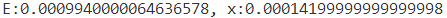
\includegraphics{Figures/del1_1d_1.png}
    \end{figure}
    \item $E\leq 0.001$ ved  $\Delta x \leq 0.0028$
    \begin{figure}[h]
    \centering
    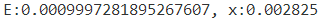
\includegraphics{Figures/del1_1d_2.png}
    \end{figure}
    \item $E\leq 0.001$ ved  $\Delta x \leq 0.032$
    \begin{figure}[h]
    \centering
    
\includegraphics{Figures/del1_1d_3.png}
    \end{figure}
    \item $E\leq 0.001$ ved  $\Delta x \leq 0.27$
    \begin{figure}[h!]
    \centering
    
\includegraphics{Figures/del1_1d_4.png}
    \end{figure}
\end{enumerate}
\newpage

\subsection{Oppgave 2}
Plott grafen til følgende funksjoner i intervallet fra tabellen over:\\
Notat: Plotting er gjort med python bibloteket matplotlib og den tilhørende pyplot klassen.
Plotting er gjort ved å lage en liste med 1000 x-verdier i intervallet for så å regne $f(x), f'(x), g(x)$ eller $E(x)$ på dem alle.
Pyplot lar oss tegne disse punktene som en rekke punkter med linjesegmenter mellom seg, eller som en rekke punkter. Vi har valgt å tegne grafene som en sum av linjesegmenter av visuelle grunner.
    \subsubsection{A)} $f(x).$
        \begin{figure}[h!]
            \begin{tabular}{cc}
            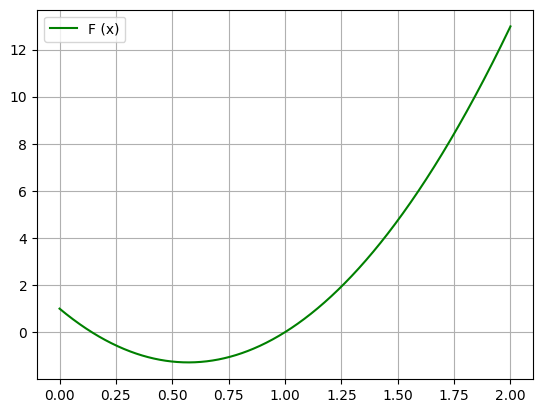
\includegraphics[width=75mm]{Figures/del1_2a_1.png} &   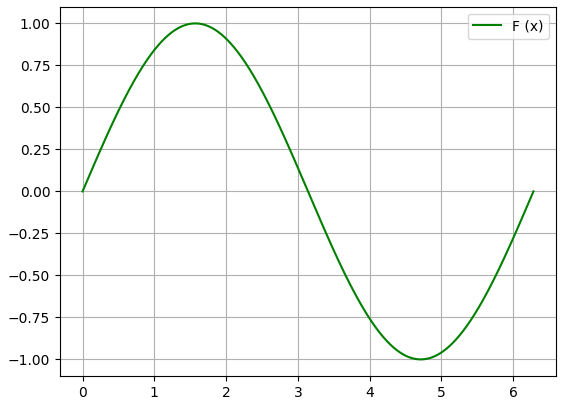
\includegraphics[width=75mm]{Figures/del1_2a_2.png} \\
            $f(x)=7x^{2}-8x+1$ & $f(x)=sin(x)$ \\[6pt]
            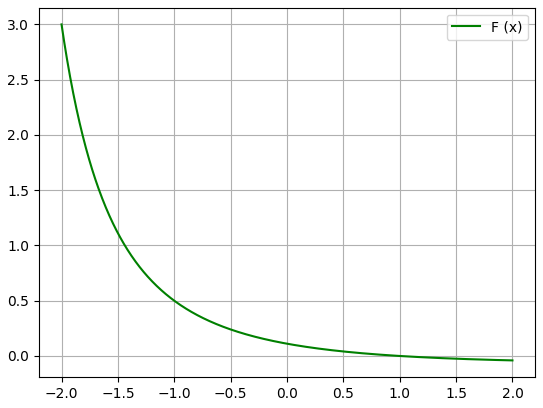
\includegraphics[width=75mm]{Figures/del1_2a_3.png} &   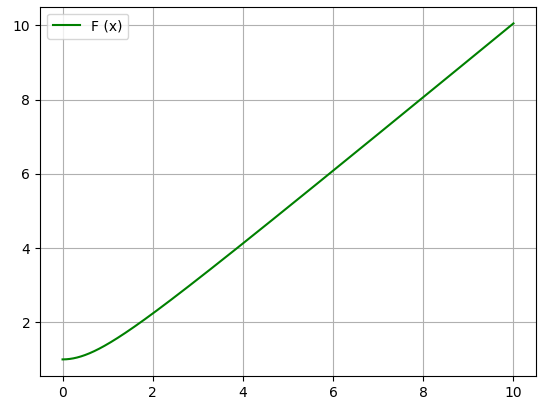
\includegraphics[width=75mm]{Figures/del1_2a_4.png} \\
            $f(x)=\frac{1-x}{(x+3)^{2}}$ & $f(x)=\sqrt{1+x^{2}}$ \\[6pt]
            \end{tabular}
        \end{figure}
        \newpage
    \subsubsection{B)} $f'(x)$
        \begin{figure}[h!]
            \begin{tabular}{cc}
            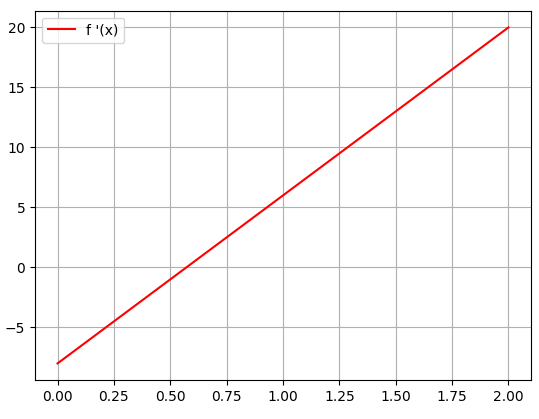
\includegraphics[width=75mm]{Figures/del1_2b_1.png} &   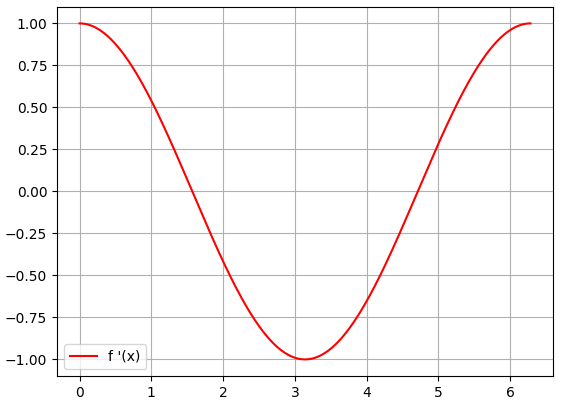
\includegraphics[width=75mm]{Figures/del1_2b_2.png} \\
            $f'(x)=14x-8$ & $f'(x)=cos(x)$ \\[6pt]
            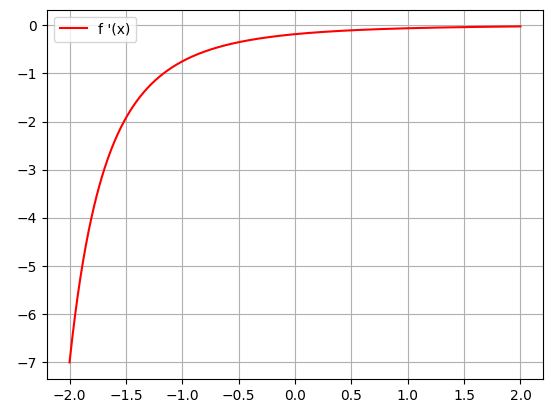
\includegraphics[width=75mm]{Figures/del1_2b_3.png} &   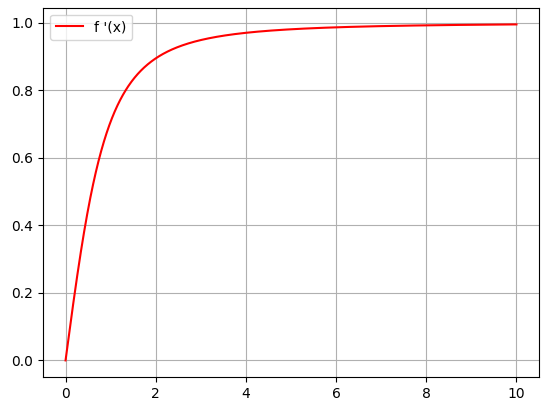
\includegraphics[width=75mm]{Figures/del1_2b_4.png} \\
            $f'(x)=\frac{x-5}{(x+3)^{3}}$ & $f'(x)=\frac{x}{\sqrt{(1+x)^{2}}}$ \\[6pt]
            \end{tabular}
        \end{figure}
        \newpage
    \subsubsection{C)} Tilnærmingen $g(x)$ med $\Delta x$ verdien fra Oppgave 1 d.
        \begin{figure}[h!]
            \begin{tabular}{cc}
            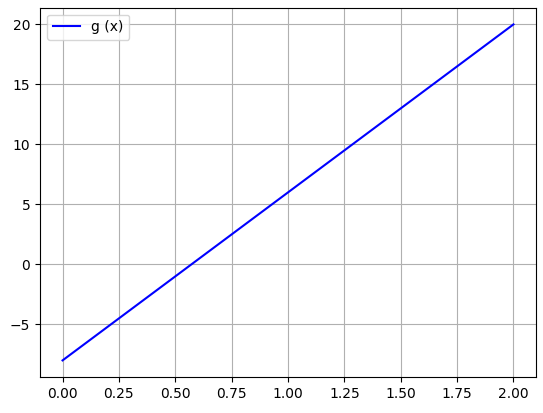
\includegraphics[width=75mm]{Figures/del1_2c_1.png} &   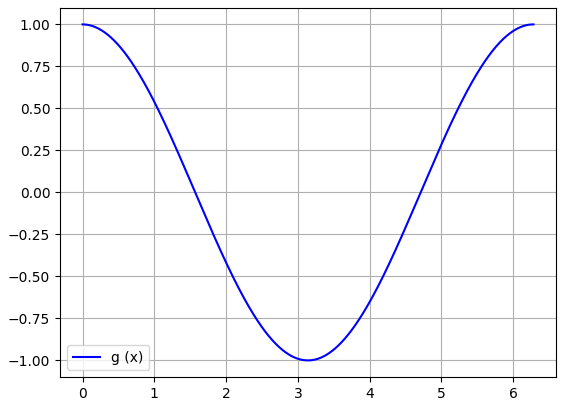
\includegraphics[width=75mm]{Figures/del1_2c_2.png} \\
            $g(x)=\frac{F(x+0.00014)-F(x)}{0.00014}$ & $g(x)=\frac{F(x+0.0028)-F(x)}{0.0028}$\\[6pt]
            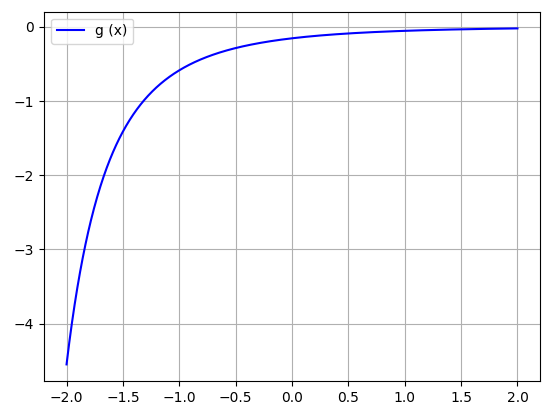
\includegraphics[width=75mm]{Figures/del1_2c_3.png} &   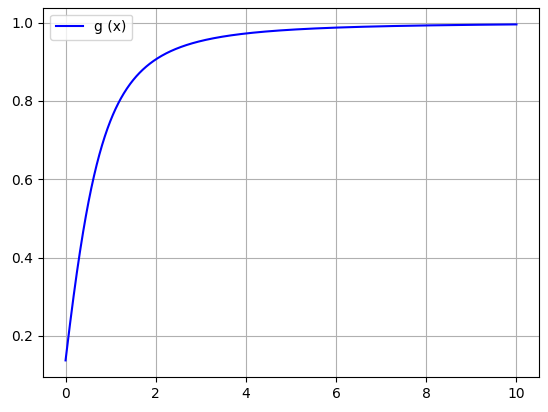
\includegraphics[width=75mm]{Figures/del1_2c_4.png} \\
            $g(x)=\frac{F(x+0.032)-F(x)}{0.032}$ & $g(x)=\frac{F(x+0.27)-F(x)}{0.27}$\\[6pt]
            \end{tabular}
        \end{figure}
        \newpage
    \subsubsection{D)} Feilen $E(x)=|f'(x) - g(x)|$\\
    MERK: I figuren for Funksjon 1 skal feilen være konstant. Variasjonen vi ser i grafen her er grunnet tallstøy/avrundingsproblemer og unøyaktigheter hos datamaskinen ved utregning av tall med mange desimaler.\\
        \begin{figure}[h!]
            \begin{tabular}{cc}
            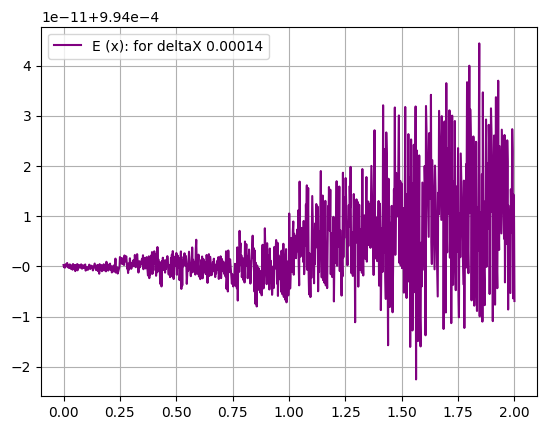
\includegraphics[width=75mm]{Figures/del1_2d_1.png} &   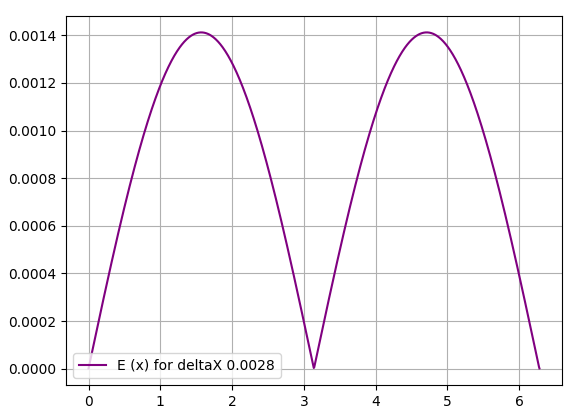
\includegraphics[width=75mm]{Figures/del1_2d_2.png} \\
            $E(x)=|f'(x) - \frac{F(x+0.00014)-F(x)}{0.00014}|$ & $E(x)=|f'(x) - \frac{F(x+0.0028)-F(x)}{0.0028}|$\\[6pt]
            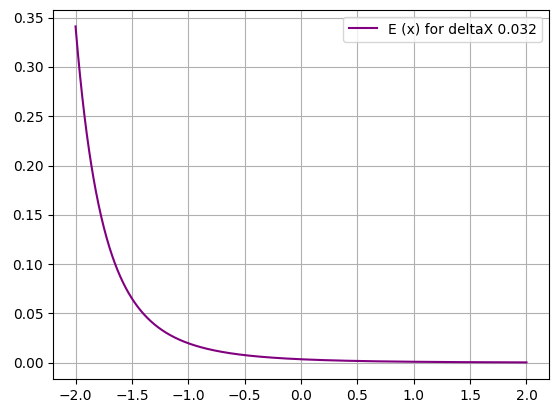
\includegraphics[width=75mm]{Figures/del1_2d_3.png} &   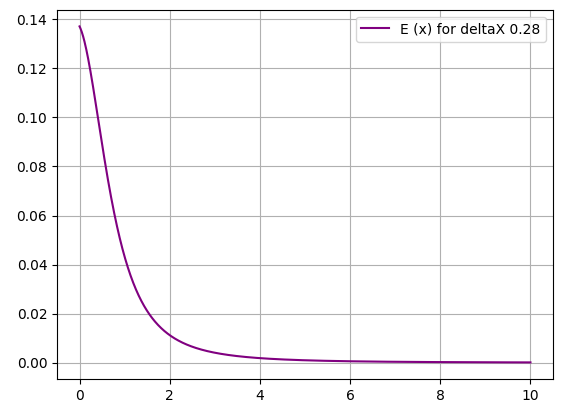
\includegraphics[width=75mm]{Figures/del1_2d_4.png} \\
            $E(x)=|f'(x) - \frac{F(x+0.032)-F(x)}{0.032}|$ & $E(x)=|f'(x) - \frac{F(x+0.27)-F(x)}{0.27}|$\\[6pt]            
            \end{tabular}
        \end{figure}
        

\section{Del 2}
\subsection{Oppgave 1}
Etter vi har satt inn $f(x)$ og $f'(x)$ ser vi at programmet konvergerer mot disse nullpunktene:
\begin{figure}[h!]
    \centering
    \begin{minipage}{0.45\textwidth}
        \centering
        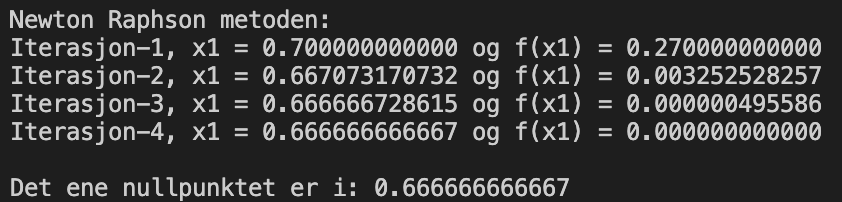
\includegraphics[width=0.9\textwidth]{Figures/del2_1_2.png}
        \caption{Startverdi: 1}
    \end{minipage}\hfill
    \begin{minipage}{0.45\textwidth}
        \centering
        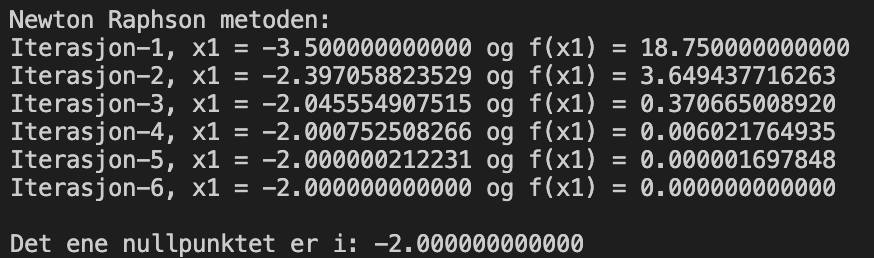
\includegraphics[width=0.9\textwidth]{Figures/del2_1_1.png}
        \caption{Startverdi: -1}
    \end{minipage}
\end{figure}
\newpage
I denne oppgaven er det bare 2 nullpunkter som du kan se på grafen av likningen under:

\begin{figure}[h!]
    \centering
    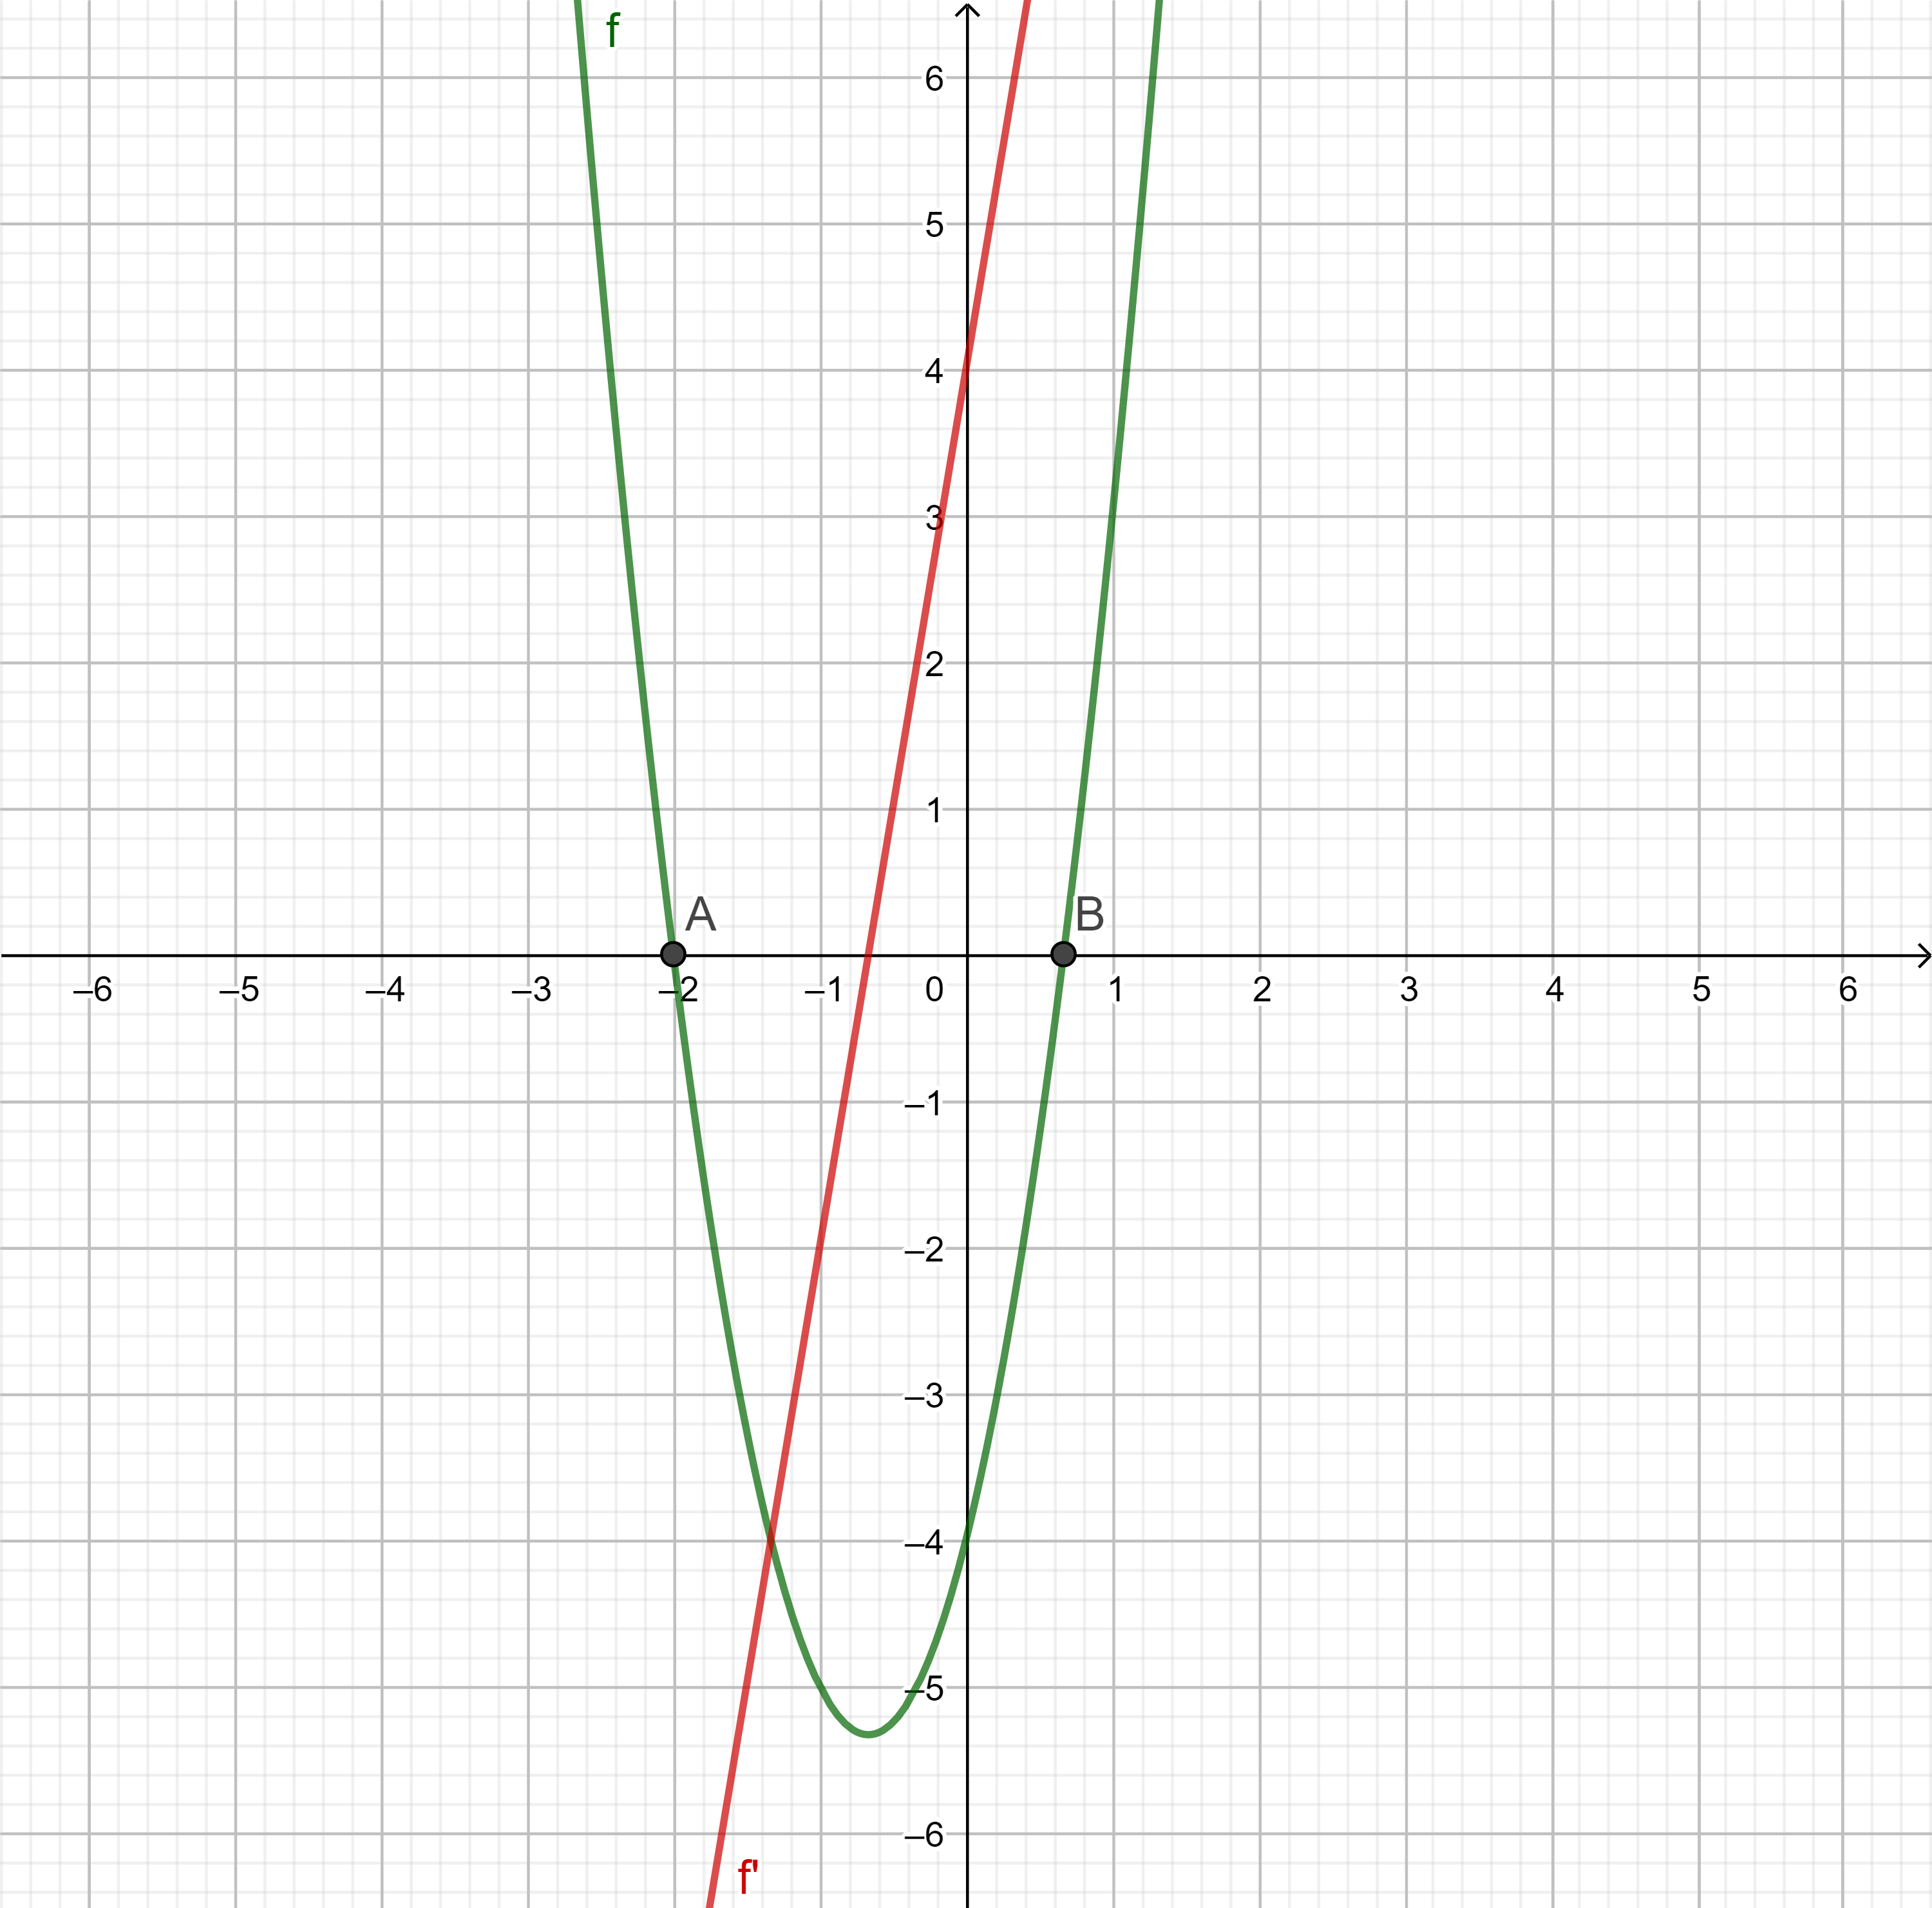
\includegraphics[width=0.40\textwidth]{Figures/Del2_1.png}
    \caption{Graf til oppgave 1, del 2}
    \label{fig:my_label}
\end{figure}

\subsection{Oppgave 2}
\subsubsection{a)}
Utledningen av likningen i denne deloppgaven:

\begin{figure}[h!]
    \centering
    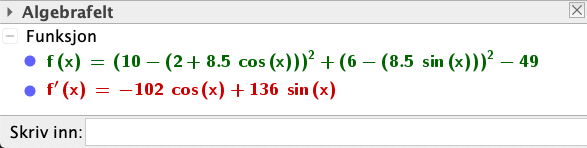
\includegraphics[width = 0.6\textwidth]{Figures/del2_2a_utledning.png}
    \caption{Utledningen gjort i GeoGebra}
    \label{fig:my_label}
\end{figure}

Etter at vi har satt inn $f(\theta_2)$ og $f'(\theta_2)$ ser vi at programmet konvergerer mot disse nullpunktene:

\begin{figure}[h!]
    \centering
    \begin{minipage}{0.45\textwidth}
        \centering
        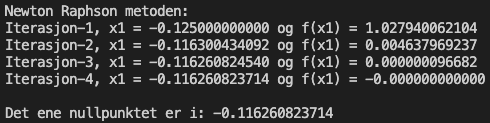
\includegraphics[width=0.9\textwidth]{Figures/del2_2a_1.png}
        \caption{Startverdi: 0}
    \end{minipage}\hfill
    \begin{minipage}{0.45\textwidth}
        \centering
        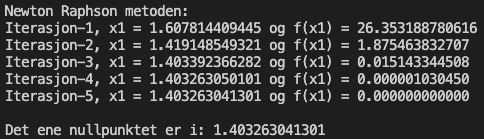
\includegraphics[width=0.9\textwidth]{Figures/del2_2a_2.png}
        \caption{Startverdi: 1}
    \end{minipage}
\end{figure}

Siden denne likningen er trigonometrisk gjelder det også for alle nullpunktene $+2k\pi$ der 'k' er større enn null og en integer. Altså for hver gang leddet i $\theta_1$ gjør en full rotasjon, kommer $\theta_2$ tilbake til samme vinkel. %Er det en bedre måte å skrive dette på?

\newpage
\subsubsection{b)}
Utledningen av likningen i denne deloppgaven:

\begin{figure}[h!]
    \centering
    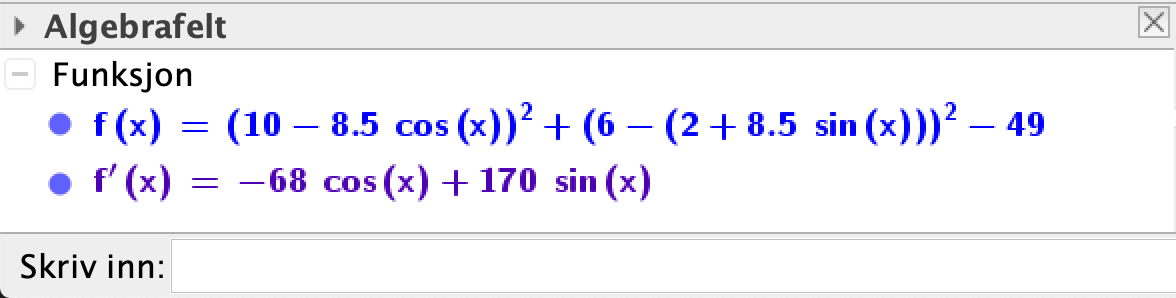
\includegraphics[width = 0.6\textwidth]{Figures/del2_2b_utledning.png}
    \caption{Utledningen gjort i GeoGebra}
    \label{fig:my_label}
\end{figure}

Etter at vi har satt inn $f(\theta_2)$ og $f'(\theta_2)$ ser vi at programmet konvergerer mot disse nullpunktene:

\begin{figure}[h!]
    \centering
    \begin{minipage}{0.45\textwidth}
        \centering
        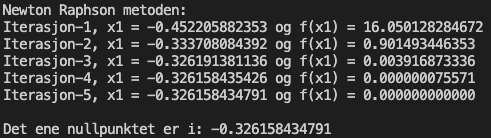
\includegraphics[width=0.9\textwidth]{Figures/del2_2b_1.png}
        \caption{Startverdi: 0}
    \end{minipage}\hfill
    \begin{minipage}{0.45\textwidth}
        \centering
        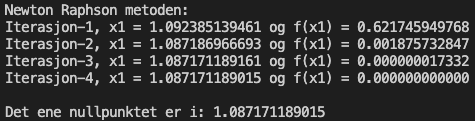
\includegraphics[width=0.9\textwidth]{Figures/del2_2b_2.png}
        \caption{Startverdi: 1}
    \end{minipage}
\end{figure}

Siden denne likningen er trigonometrisk gjelder det også for alle nullpunktene $+2k\pi$ der 'k' er større enn null og en integer. Altså for hver gang leddet i $\theta_1$ gjør en full rotasjon, kommer $\theta_2$ tilbake til samme vinkel. %Er det en bedre måte å skrive dette på?

\subsubsection{c)}
Utledningen av likningen i denne deloppgaven:

\begin{figure}[h!]
    \centering
    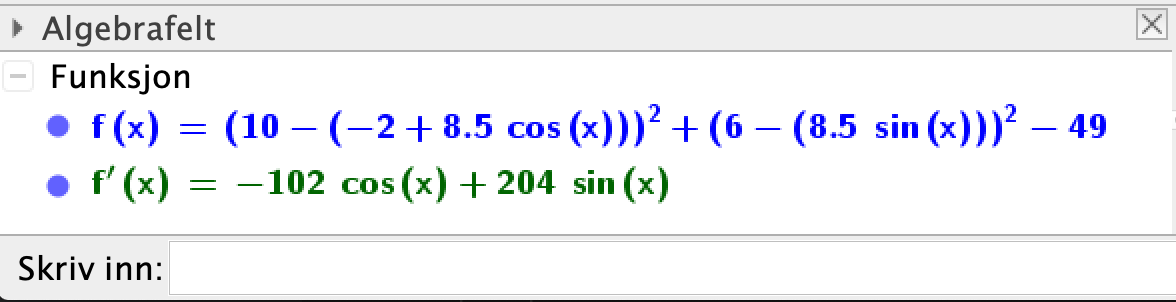
\includegraphics[width = 0.6\textwidth]{Figures/del2_2c_utledning.png}
    \caption{Utledningen gjort i GeoGebra}
    \label{fig:my_label}
\end{figure}

Etter at vi har satt inn $f(\theta_2)$ og $f'(\theta_2)$ ser vi at programmet konvergerer mot disse nullpunktene:

\begin{figure}[h!]
    \centering
    \begin{minipage}{0.45\textwidth}
        \centering
        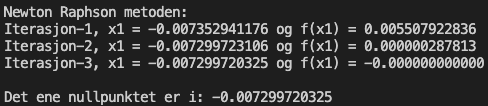
\includegraphics[width=0.95\textwidth]{Figures/del2_2c_1.png}
        \caption{Startverdi: 0}
    \end{minipage}\hfill
    \begin{minipage}{0.45\textwidth}
        \centering
        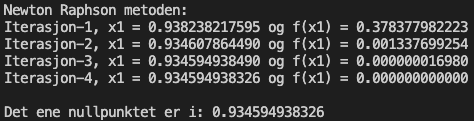
\includegraphics[width=0.9\textwidth]{Figures/del2_2c_2.png}
        \caption{Startverdi: 1}
    \end{minipage}
\end{figure}

Siden denne likningen er trigonometrisk gjelder det også for alle nullpunktene $+2k\pi$ der 'k' er større enn null og en integer. Altså for hver gang leddet i $\theta_1$ gjør en full rotasjon, kommer $\theta_2$ tilbake til samme vinkel. %Er det en bedre måte å skrive dette på? 
 